\documentclass[12pt]{article}

% LuaLaTeX basics
\usepackage{fontspec}
\usepackage{amsmath}
\usepackage{mathtools}
\usepackage{unicode-math}
% Fonts (Libertine-Äquivalent, modern)
\setmainfont{Libertinus Serif}
\setsansfont{Libertinus Sans}
\setmonofont{Libertinus Mono}

% Layout & typography
\usepackage[a4paper]{geometry}
\usepackage{setspace}
\usepackage{parskip}
\usepackage{graphicx}
\usepackage{amsmath}
\usepackage{booktabs}
\usepackage{tabularx}

% Chemistry
\usepackage{chemfig}
\usepackage[modules]{chemmacros}
\usepackage{siunitx}
\chemsetup{
  modules = {
    reactions,
    spectroscopy,
    scheme
  },
  formula = mhchem
}
\usepackage{fancyhdr}
\usepackage{overcite}
\usepackage{hyperref}
\usepackage{tabulary}


\usepackage[ddmmyyyy]{datetime}
\renewcommand{\dateseparator}{.}
\usepackage{overcite}
\renewcommand\citeform[1]{[#1]}


\newcommand\textbox[1]{%
  \parbox{.333\textwidth}{#1}%
}

\pagestyle{fancy}

\cfoot{\thepage}

\lhead{Nevroz Arslan }
\rhead{\today}
\setlength{\headheight}{15pt}

\renewcommand{\thesection}{\arabic{section}.}
\renewcommand{\thesubsection}{\thesection\arabic{subsection}}
\renewcommand{\headrulewidth}{0pt}

\begin{document}

\begingroup
\leftskip=0cm plus 0.5fil \rightskip=0cm plus -0.5fil
\parfillskip=0cm plus 1fil
 \textbf{\large Darstellung von Ferrocenaldehyd}\par
\endgroup

\begin{center}
 \textbf{Präparat Nr. 2 von 4}
\end{center}
\section{Reaktionstyp: \textnormal{Vilsmeier-Haack-Reaktion} }
\begin{figure}[ht]
\centering
\includegraphics[width=\textwidth]{reaktion.png}
\end{figure}

\begin{onehalfspace}

\section{Berechnung des Ansatzes: }
Es sollte aus 5.300 g (28.49 \si{\milli\mol}) Ferrocen Ferrocenaldehyd hergestellt werden.
Die Umrechnung des Literaturansatzes\cite{bio} ergab folgenden Ansatz:\\[0.5cm]
\begin{tabularx}{\textwidth}{lrrrr}
\toprule
\textbf{Bezeichnung}&\textbf{ M [\si{\gram\per\mol}]} & \textbf{n [\si{\milli\mol}]} & \textbf{Menge} & \textbf{Equiv}\\
\midrule
Ferrocen & 186.04 & 28.5  &  5.3 \si{\gram} &1.00   \\
Phosphoroxychlorid  & 153.32 & 115.0  & 10.5 \si{\milli\liter} & 4.10   \\
Dimethylformamid     & 73.10  & 195.0  & 15.0 \si{\milli\liter} & 6.84   \\
Chloroform     &  &  &  & LM   \\
\bottomrule
\end{tabularx}

\normalsize \section{Durchführung \cite{bio}}
In einem 250 \si{\milli\liter} Dreihalskolben, ausgestattet mit Tropftrichter und Rückflusskühler, wurde Ferrocen (5.3 g, 28 \si{\milli\mol}) in Chloroform (60 \si{\milli\liter}) vorgelegt und mit Hilfe eines Salz-Eisbades auf -5 \si{\celsius} gekühlt. Im Anschluss wurde Phosphoroxychlorid (10.5 \si{\milli\liter}, 115.0 \si{\milli\mol}) in Dimethylformamid (15 \si{\milli\liter}, 195.0 \si{\milli\mol}) gelöst und durch einen Tropftrichter innerhalb von zwei Stunden  hinzugegeben. Das Reaktionsgemisch wurde danach 12 Stunden unter Rückfluss gerührt. Nach beendetem Refluxieren wurde das Reaktionsgemisch durch Kältedestillation zur Trockne gedampft. Der Rückstand wurde mit Eis-Wasser (100 \si{\milli\liter}) hydrolysiert und abfiltriet. Das so erhaltene Filtrat wurde mit \ce{NaOH} (10\%-ige, 100 \si{\milli\liter}) auf pH 8 neutralisiert und mit Ether (150 \si{\milli\liter}) extrahiert. Die organische Phase wird mit Wasser gewaschen und über \ce{MgSO_4} getrocknet. Nach dem Entfernen des Lösungsmittels wurde das Produkt aus n-Hexan kristallisiert. Das Produkt (0.312 \si{\gram}, 1.46 \si{\milli\mol}, 5 \%) wurde als dunkelroter Feststoff erhalten.

\section{Ausbeute}
\begin{tabular}{ll}
  6.020 \si{\gram} (28 \si{\milli\mol}) =  & 100 \%\\
  0.312 \si{\gram} (1.46 \si{\milli\mol}) =  & 5 \% (Lit.\cite{bio} : 79 \%) \\
\end{tabular}
\newpage
\section{Spektrenauswertung}
\begin{figure}[!ht]
   \centering
\includegraphics[scale=0.3]{auswert.png}
\end{figure}
\noindent
\textbf{\ce{^1_{}H-NMR}} (300 MHz, \ce{CDCl_3}): \ce{$\delta$} = 
4.22 (s, 5 H, 5-H),
4.55 (s, 2 H, 4-H),
4.73 (s, 2~H, 3-H),
9.92 (s, 1 H, 1-H) ppm.
\section{Mechanismus\cite{mech}\cite{mech2}}
Im ersten Teil der Reaktion wird das Formylierungsreagenz aus Dimethylformamid (\textbf{1}) und Phosphoroxychlorid (\textbf{2}) generiert.
Dazu greift zunächst das Sauerstoff-Atom des Dimethylformamids (\textbf{1}) das Phosphoroxychlorids (\textbf{2}) an.
Es bildet sich dabei ein Phosphoesterimminium-Zwischenstufe \textbf{3}, welche unter Abspaltung des Dichloridodioxophosphats in ein Iminiumion \textbf{3} umgewandelt.
Im zweiten Teil der Reaktion erfolgt eine sogennante Vilsmeier-Reaktion.
Das Iminiumion \textbf{3} reagiert in einer elektrophilen aromatischen Substitutionsreaktion mit dem Ferrocen (\textbf{5}).
Es bildet sich unter Aufhebung der Aromatizität des Benzolrings ein Arenium-Ion \textbf{6}.  
Unter Deprotonierung des Arenium-Ions \textbf{6} findet eine Rearomatisierung statt. Das so enstandene Zwischenprodukt \textbf{7}
wird unter Abspaltung des Chlorids in ein Ferrocenimminum-Ion \textbf{7} überführt, welches durch Hydrolyse das gewünschte Produkt (\textbf{8}) ergibt. 
\newpage
\begin{figure}[!ht]
   \centering
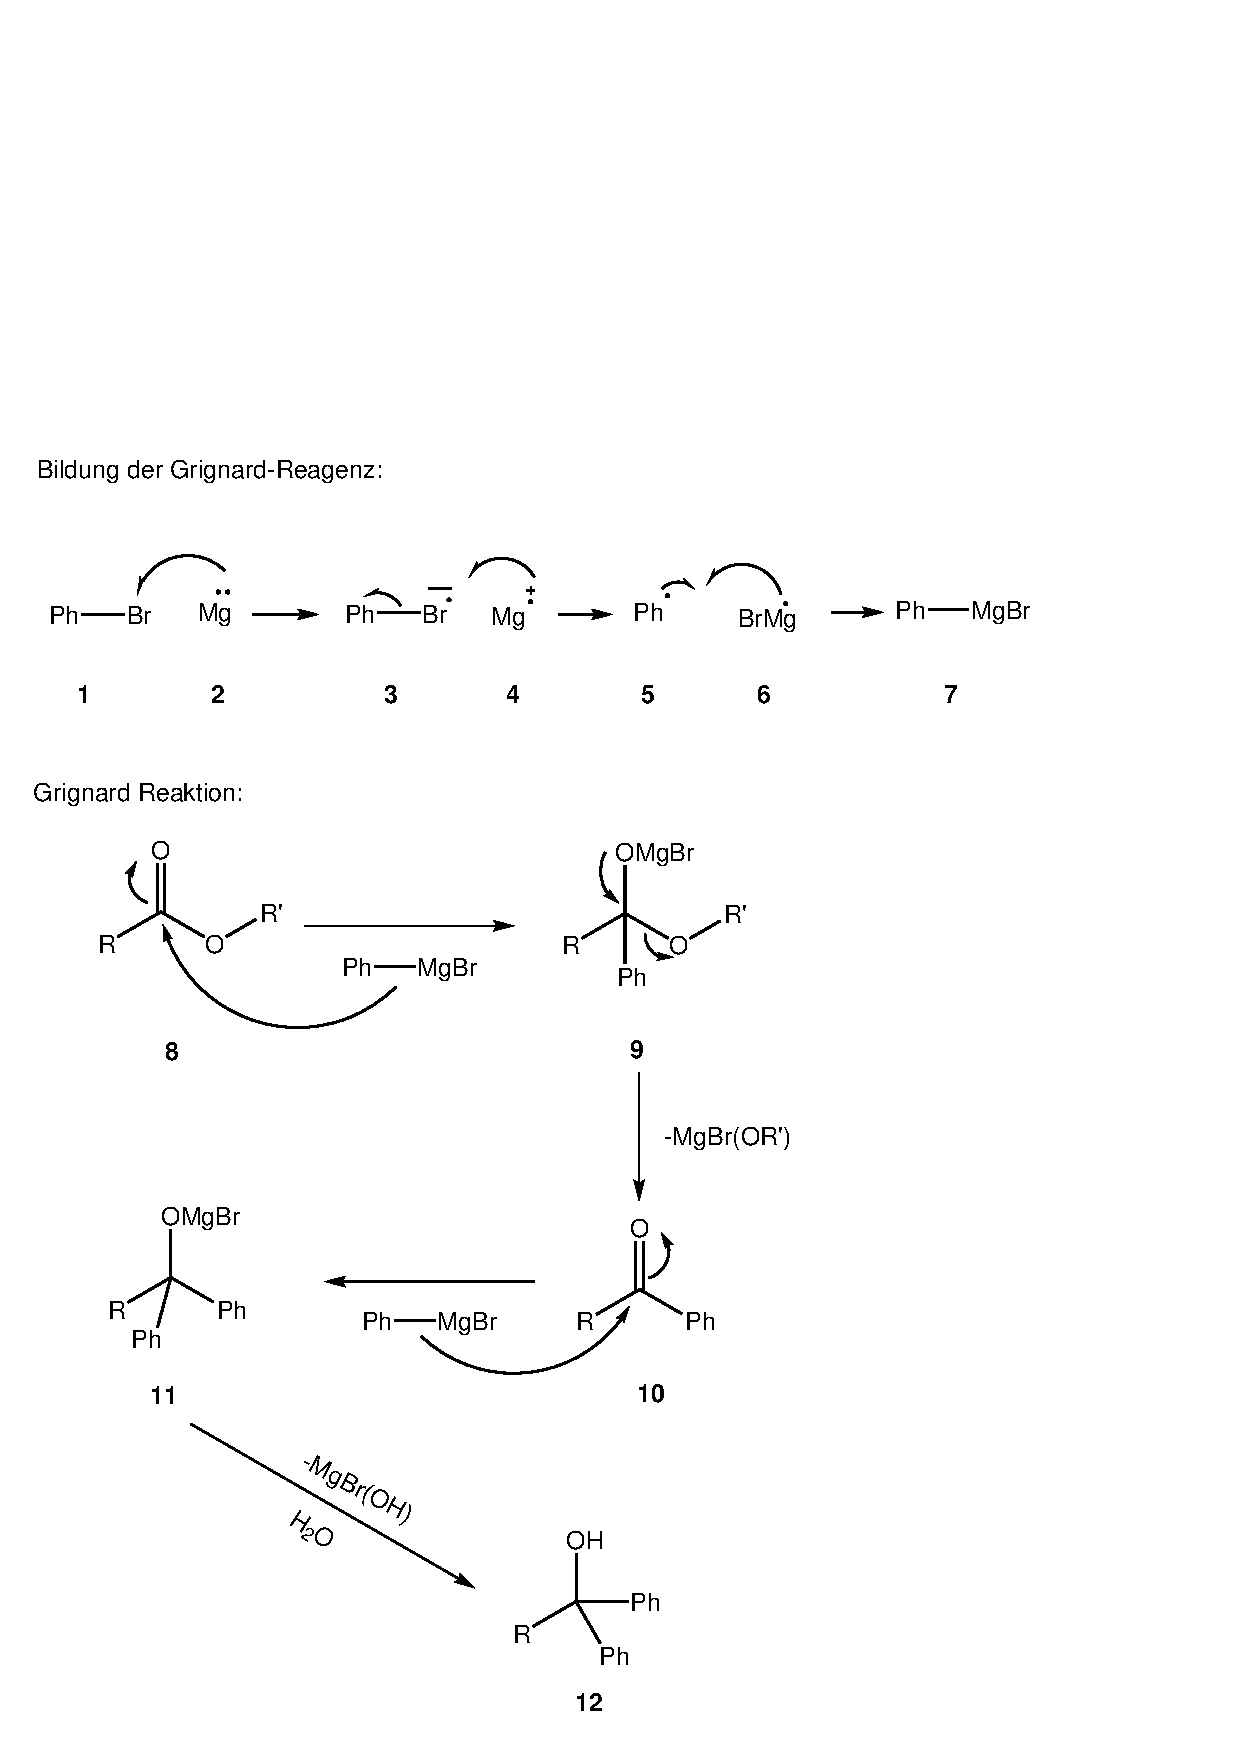
\includegraphics[width=\textwidth]{mechan.png}
\end{figure}
\section{Abfallentsorgung}
Die nach dem Hydrolysieren verbleibenden wässrigen Phasen wurden
nach einer pH-Wertbestimmung im Behälter für basische wässrige Abfälle entsorgt.
Das abgetrennte Lösungsmittel wurde im Behälter für halogenhaltige Kohlenwasserstoffe entsorgt.
\section{Literatur}
\renewcommand{\section}[2]{}%
\begin{thebibliography}{}
\bibitem{bio}
J. Jia, Y. Cui, Y. Li, W. Sheng, L. Han, J. Gao, \textit{Dyes and Pigments} \textbf{2013}, 9, 273 - 279.
\bibitem{mech}
T. Laue, A. Plagens, \textit{Namen- und Schlagwortreaktionen der Organischen Chemie}, 4. Aufl., Teubner, Stuttgart \textbf{2006}, S. 330-331.
\bibitem{mech2}
J. Buddrus, \textit{Grundlagen der Organische Chemie}, 4. Aufl., De Gruyter, Berlin \textbf{2011}, S. 358.
\end{thebibliography}
\end{onehalfspace}
\end{document}